\subsubsection{BJT tipo NPN e PNP}

Os transistores bipolares de junção (BJT -- Bipolar Junction Transistor) são dispositivos semicondutores cujo funcionamento depende do controle da corrente entre dois terminais por meio de uma corrente aplicada ao terceiro terminal.

Diferentemente dos MOSFETs, que utilizam um campo elétrico para controlar a formação de um canal condutor, os BJTs utilizam o movimento de elétrons e lacunas através de duas junções semicondutoras.

Sua estrutura é composta por três regiões:


\textbf{Emissor (Emitter):} região responsável por fornecer os portadores de carga.
\textbf{Base (Base):} região intermediária, muito fina, responsável por controlar o fluxo de portadores.
\textbf{Coletor (Collector):} região responsável por coletar os portadores que atravessam a base.


Existem dois tipos principais de transistores BJT:

\begin{figure}[H]
    \centering
    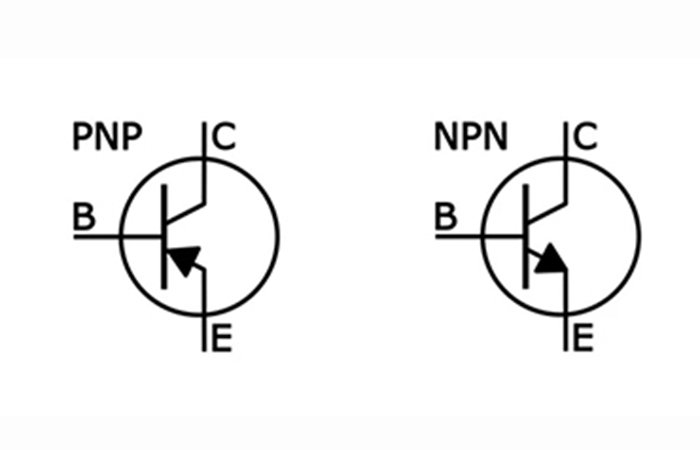
\includegraphics[width=0.6\linewidth]{images/npn-pnp-transistors.jpg}
    \caption{Representação dos transistores BJT tipo NPN e PNP}
    \label{npn-pnp-transistors}
    {\footnotesize Fonte: \url{https://www.langirswitch.com}}
\end{figure}


\textbf{NPN:} possui duas regiões do tipo N separadas por uma região do tipo P. Quando a junção base-emissor é polarizada diretamente, permitindo a injeção de elétrons do emissor para a base, e a junção base-coletor é polarizada reversamente, a maior parte desses elétrons atravessa a base e é coletada pelo coletor. Dessa maneira, uma pequena corrente de base controla uma corrente significativamente maior entre coletor e emissor.

\textbf{PNP:} apresenta uma estrutura complementar, com duas regiões do tipo P separadas por uma região do tipo N. Nesse caso, os principais portadores de carga são as lacunas, que são injetadas pelo emissor e atravessam a base em direção ao coletor. O transistor é ativado quando a base apresenta uma tensão suficientemente inferior à tensão do emissor.

\paragraph{Funcionamento físico do BJT NPN}

\begin{figure}[H]
    \centering
    \includegraphics[width=0.6\linewidth]{images/npn.jpg}
    \caption{Diagrama do transistor NPN de junção}
    \label{npn-diagram}
    {\footnotesize Fonte: \url{https://thescienceplus.com/news/data/20221221/p1065576011314123_8983_thum.jpg}}
\end{figure}

Para compreender o funcionamento de um transistor NPN, considere sua estrutura formada por um emissor do tipo N, uma base do tipo P e um coletor do tipo N.

Quando a tensão entre base e emissor ($V_{BE}$) é suficientemente positiva, a junção base-emissor fica diretamente polarizada. Em um transistor de silício operando em condições usuais, essa tensão costuma estar próxima de 0,7 V, embora não seja um valor fixo ou universal.

Essa polarização permite que elétrons sejam injetados pelo emissor na região da base. Como a base é extremamente fina e geralmente possui baixa concentração de dopagem em comparação ao emissor, apenas uma pequena parcela desses elétrons se recombina com lacunas presentes na base.

A maior parte dos elétrons atravessa a base e alcança a junção base-coletor, que normalmente está reversamente polarizada. O campo elétrico nessa região conduz os elétrons em direção ao coletor.

Como resultado, uma pequena corrente de base controla uma corrente muito maior entre coletor e emissor.

Na região ativa do transistor, essa relação pode ser aproximada por:

\[
I_C \approx \beta I_B
\]

Onde:

\begin{itemize}
    \item $I_C$: corrente de coletor;
    \item $I_B$: corrente de base;
    \item $\beta$: ganho de corrente do transistor.
\end{itemize}

O parâmetro $\beta$, também denominado $h_{FE}$, representa a relação entre a corrente de coletor e a corrente de base. Seu valor depende do transistor e das condições de operação.

\paragraph{Funcionamento físico do BJT PNP}

O transistor PNP apresenta um funcionamento complementar ao NPN. Nesse caso, os principais portadores de carga são as lacunas.

Quando a tensão da base é suficientemente inferior à tensão do emissor, a junção base-emissor fica diretamente polarizada, permitindo a injeção de lacunas do emissor para a base.

Assim como ocorre no NPN, a pequena espessura da base faz com que a maior parte dos portadores atravesse essa região e alcance o coletor.

A corrente convencional flui do emissor para o coletor, enquanto a corrente de base sai do transistor.

A relação entre as correntes também pode ser aproximada por:

\[
I_C \approx \beta I_B
\]

Considerando os sentidos convencionais das correntes e utilizando seus módulos.

\paragraph{Regiões de operação do BJT}

O BJT pode operar em diferentes regiões, dependendo das tensões aplicadas às suas junções:


\textbf{Corte:} ambas as junções estão sem polarização direta significativa. A corrente de coletor é praticamente nula, e o transistor se comporta como uma chave aberta.
    
\textbf{Região ativa:} a junção base-emissor está diretamente polarizada e a junção base-coletor está reversamente polarizada. Nessa condição, o transistor funciona como amplificador, pois pequenas variações na corrente de base produzem variações maiores na corrente de coletor.
    
\textbf{Saturação:} ambas as junções estão diretamente polarizadas. O transistor conduz intensamente e apresenta uma pequena tensão entre coletor e emissor, comportando-se aproximadamente como uma chave fechada.
